%!TEX root = ../main.tex
\chapter{Hypothesentests}
\section{Allgemeines zu Tests und Hypothesen}
Es ist immer ein Signifikanzniveau $\alpha$ gegeben, mit dem man den Fehler 1. Art beschränkt.

\subsection{Links- rechtsseitiger Hypothesentest}
Für einen Binomialtest um $p\in\Theta=(0,1)$ zu testen sehen die wichtigen Werte in etwa so aus
\begin{center}
	\begin{tabular}{r|ccc}
		&linksseitig&gemeinsam&rechtsseitig\\\hline
		Annahmebereich:&$\Theta_0=[p_0,1)$&$\Big|$&$\Theta_0=(0,p_0]$\\
		Ablehnungsbereich:&&$\Theta_1=(0,1)\setminus\Theta_0$&\\
		Kritischer Punkt:&\makecell{$k^\ast$ maximal mit\\ $P_{p_0}(X\leq k^\ast)\leq\alpha$}&$\Bigg|$&\makecell{$k^\ast$ minimal mit\\ $P_{p_0}(X\geq k^\ast)\leq\alpha$}\\
		Kritischer Bereich:&$\mathcal K_1=\simpleset{0,\ldots,k^\ast}$&$\Big|$&$\mathcal K_1=\simpleset{k^\ast,\ldots,n}$\\
		Gütefunktion:&&$g(\theta)=P_\theta(X\in\mathcal K_1)$&\\
		Signifikanzniveau:&&$\alpha>0$&
	\end{tabular}
\end{center}

Eine Gütefunktion für einen rechtsseitigen Test steigt nach rechts an, eine für einen linksseitigen Test fällt von links ab. D.h. immer im Annahmebereich $\Theta_0$ ist sie klein.

Gütefunktion für einen rechtsseitigen Test
\begin{center}
	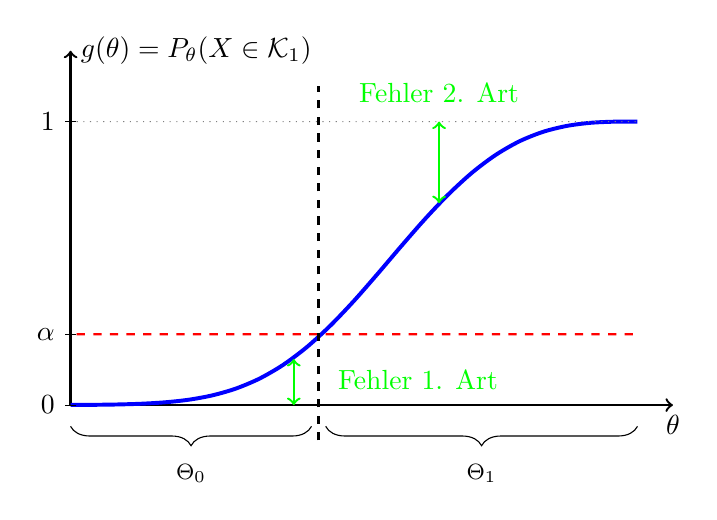
\begin{tikzpicture}[scale=0.9]
		\draw[->, line width=0.3mm] (0,0) to (8.5,0) node[below] {$\theta$};
		\draw[->, line width=0.3mm] (0,0) to (0,5) node[right] {$g(\theta)=P_\theta(X\in \mathcal K_1)$};		

		\draw[line width=0.5mm,scale=1,domain=0:8,smooth,variable=\x,blue] plot ({\x},{4*exp((\x/4-2)^3)});
		%\draw[line width=0.5mm,scale=1,domain=4:8,smooth,variable=\x,blue] plot ({\x},{-3.12*exp(-(\x-4))+4});
		
		\draw (0,0) node (null) [rectangle,inner sep = 0pt,minimum size = 0pt,minimum width=4pt,draw, label={left:$0$}] {};
		\draw (0,4) node (eins) [rectangle,inner sep = 0pt,minimum size = 0pt,minimum width=4pt,draw, label={left:$1$}] {};
		\draw (0,1) node (alpha) [rectangle,inner sep = 0pt,minimum size = 0pt,minimum width=4pt,draw, label={left:$\alpha$}] {};

		\draw[red, dashed, line width=0.3mm] (alpha) -- (8,1);
		\draw[gray, dotted] (eins) -- (8,4);

		\draw[black, line width=0.3mm, dashed] (3.5,-0.5) -- (3.5,4.5);
			
		\draw [decorate,decoration={brace,amplitude=7pt}]
		(3.4,-0.3) -- (0,-0.3) node [black,midway, yshift=-17pt] 
		{\footnotesize $\Theta_0$};

		\draw [decorate,decoration={brace,amplitude=7pt}]
		(8,-0.3) -- (3.6,-0.3) node [black,midway, yshift=-17pt] 
		{\footnotesize $\Theta_1$};

		%Fehler 1. Art
		\draw [arrows=<->, green, line width=0.3mm] (3.15,0) -- (3.15,0.65);
		\draw (3.5,0.35) node (null) [label={right:{\color{green}Fehler 1. Art}}] {};
		

		%Fehler 2. Art
		\draw [arrows=<->, green, line width=0.3mm] (5.2,2.85) -- (5.2,4);
		\draw (5.2,4) node (null) [label={above:{\color{green}Fehler 2. Art}}] {};
		
		
	\end{tikzpicture}	
\end{center}

\subsection{Fehlerarten}
\begin{center}
	\begin{tabular}{r|cc}
		&$H_0$ gilt&$H_1$ gilt\\\hline
		$H_0$ nicht abgelehnt&Spezifität&\makecell{Fehler 2. Art\\ false negative}\\
		$H_0$ abgelehnt&\makecell{Fehler 1. Art\\ false positive}&Sensitivität
	\end{tabular}
\end{center}
Der Fehler erster Art beschreibt die Wahrscheinlichkeit, die Nullhypothese fälschlicherweise abzulehnen
\begin{equation*}
	P_{\theta_0}(X\in \mathcal K_1)
\end{equation*}

Der Fehler zweiter Art beschreibt die Wahrscheinlichkeit, die Nullhypothese fälschlicherweise anzunehmen (nicht zu verwerfen)
\begin{equation*}
	P_{\theta_1}(X\in \mathcal K_0)
\end{equation*}

\section{Binomialtest}

\section{Gaußtest (Test mit der Normalverteilung)}
Wir wollen mit dem Mittelwert der Normalverteilung einen Hypothesentest durchführen. Das heißt also zum Beispiel prüfen ob der Mittelwert tatsächlich einem erwarteten Wert $\mu$ entspricht.
\begin{enumerate}
	\item Wir verwenden hierfür die Teststatistik $\overline X=\frac1n\sum_{i=1}^n X_i$ als Schätzer für den Mittelwert. Wir benötigen außerdem den Standardfehler $\sigma_{\overline X}=\sqrt{\frac{\sigma^2}{n}}$ um auf die Standardnormalverteilung reduzieren zu können.
	\item Nun führen den Test auf eine Standardnormalverteilung zurück, indem wir die folgende Zufallsvariable festlegen
	\begin{equation*}
		Z=\frac{\overline X-\mu}{\frac{\sigma}{\sqrt n}}\sim\norm(0,1).
	\end{equation*}
	\item Wir können nun die Quantile $z_p$ der Standardnormalverteilung aus einer Tabelle ablesen.
	Dann wird der Ablehnungsbereich $\Theta_1$ entsprechend dem Signifikanzniveau $\alpha$ wie folgt bestimmt
	\begin{center}
		\begin{tabular}{c|c|c}
			linksseitiger Test&rechtsseitiger Test&beidseitiger Test\\\hline
			$\Theta_1=(-\infty, z_{\alpha}]$&$\Theta_1=[z_{1-\alpha},\infty)$&$\Theta_1=(-\infty, z_{\alpha/2}]+[z_{1-\alpha/2},\infty)$
		\end{tabular}
	\end{center}
	\item Als letztes muss man noch prüfen, ob der beobachtete Wert aus der Teststatistik im Ablehnungsbereich liegt. Das heißt, falls
	\begin{equation*}
	 	\frac{\overline X-\mu}{\frac{\sigma}{\sqrt n}}\in \Theta_1
	\end{equation*}
	für die gegebene Stichprobe gilt, so wird $H_0$ zum gegebenen Signifikanzniveau verworfen.
\end{enumerate}

\section{$\chi^2$-Anpassungstest}
